\documentclass{sig-alternate-ipsn13}

\newcommand\tabhead[1]{\small\textbf{#1}}
\usepackage{multirow}

\begin{document}

\title{Classroom Usage Detection System}
%
% You need the command \numberofauthors to handle the 'placement
% and alignment' of the authors beneath the title.
%
% For aesthetic reasons, we recommend 'three authors at a time'
% i.e. three 'name/affiliation blocks' be placed beneath the title.
%
% NOTE: You are NOT restricted in how many 'rows' of
% "name/affiliations" may appear. We just ask that you restrict
% the number of 'columns' to three.
%
% Because of the available 'opening page real-estate'
% we ask you to refrain from putting more than six authors
% (two rows with three columns) beneath the article title.
% More than six makes the first-page appear very cluttered indeed.
%
% Use the \alignauthor commands to handle the names
% and affiliations for an 'aesthetic maximum' of six authors.
% Add names, affiliations, addresses for
% the seventh etc. author(s) as the argument for the
% \additionalauthors command.
% These 'additional authors' will be output/set for you
% without further effort on your part as the last section in
% the body of your article BEFORE References or any Appendices.

\numberofauthors{1} %  in this sample file, there are a *total*
% of EIGHT authors. SIX appear on the 'first-page' (for formatting
% reasons) and the remaining two appear in the \additionalauthors section.
%
\author{
% You can go ahead and credit any number of authors here,
% e.g. one 'row of three' or two rows (consisting of one row of three
% and a second row of one, two or three).
%
% The command \alignauthor (no curly braces needed) should
% precede each author name, affiliation/snail-mail address and
% e-mail address. Additionally, tag each line of
% affiliation/address with \affaddr, and tag the
% e-mail address with \email.
%
\alignauthor Chun-Yen Hsu, Yu-Liang Hsu, Takuma Oda\\
\affaddr{Carnegie Mellon University} \\ {94035 Mountain View}\\{California, USA}\\
\email{\{chunyenh,yuliangh\}@andrew.cmu.edu\\ takuma.oda@sv.cmu.edu}
% 1st. author
% \alignauthor
% Chun-Yen Hsu\\
%        % \titlenote{Dr.~Trovato insisted his name be first.}\\
%        \affaddr{Carnegie Mellon University}\\
%        \affaddr{94035 Mountain View}\\
%        \affaddr{California, USA}\\
%        \email{chunyenh@andrew.cmu.edu}
% % 2nd. author
% \alignauthor
% Yu-Liang Hsu\\
%        % \titlenote{Dr.~Trovato insisted his name be first.}\\
%        \affaddr{Carnegie Mellon University}\\
%        \affaddr{94035 Mountain View}\\
%        \affaddr{California, USA}\\
%        \email{yuliangh@andrew.cmu.edu}
% % 3rd. author
% \alignauthor
% Takuma Oda\\
%        % \titlenote{Dr.~Trovato insisted his name be first.}\\
%        \affaddr{Carnegie Mellon University}\\
%        \affaddr{94035 Mountain View}\\
%        \affaddr{California, USA}\\
%        \email{takuma.oda@sv.cmu.edu}
% \alignauthor Lars Th{\o}rv{\"a}ld\titlenote{This author is the
% \email{larst@affiliation.org}
% \and  % use '\and' if you need 'another row' of author names
% % 4th. author
% \alignauthor Lawrence P. Leipuner\\
%        \affaddr{Brookhaven Laboratories}\\
%        \affaddr{Brookhaven National Lab}\\
%        \affaddr{P.O. Box 5000}\\
%        \email{lleipuner@researchlabs.org}
% % 5th. author
% \alignauthor Sean Fogarty\\
%        \affaddr{NASA Ames Research Center}\\
%        \affaddr{Moffett Field}\\
%        \affaddr{California 94035}\\
%        \email{fogartys@amesres.org}
% % 6th. author
% \alignauthor Charles Palmer\\
%        \affaddr{Palmer Research Laboratories}\\
%        \affaddr{8600 Datapoint Drive}\\
%        \affaddr{San Antonio, Texas 78229}\\
%        \email{cpalmer@prl.com}
}
% There's nothing stopping you putting the seventh, eighth, etc.
% author on the opening page (as the 'third row') but we ask,
% for aesthetic reasons that you place these 'additional authors'
% in the \additional authors block, viz.
\additionalauthors{Additional authors: John Smith (The Th{\o}rv{\"a}ld Group,
email: {\texttt{jsmith@affiliation.org}}) and Julius P.~Kumquat
(The Kumquat Consortium, email: {\texttt{jpkumquat@consortium.net}}).}
\date{30 July 1999}
% Just remember to make sure that the TOTAL number of authors
% is the number that will appear on the first page PLUS the
% number that will appear in the \additionalauthors section.

\maketitle
\begin{abstract}

In this paper, we present a classroom usage detection system. We put vibration sensors on each table in the room to detect the usage of a room. Due to heavy usage study table requirement in our campus, it's hard to find an available seat to study. We also want to save the energy when the room is vacant. Therefore we developed "Classroom Usage Detection System". There are 3 major steps of detecting the usage: vibration sensing, table event detection and event counting. We used several different methods to analyze the data: sequential detection model (SD), event counting model (EC) and filtered event counting model (FEC). Our system got 98\% accuracy when there someone using the table. And with approximately 83\% accuracy when there is nobody using the table.



\end{abstract}

\section{Introduction}

Heavy course workload and the pressure of finding a job make extremely high study room demand for graduate students in Carnegie Mellon University. Students usually need a great and quiet study environment not only for less noise from others but also for higher learning efficiency. However, due to the large amount of demand, students can only search for study room one by one for the sake of an available seat to read, which consumes lots of unnecessary time. In the worst case, students are not able to find a place to study. Also, students often forget to turn off the light and the heater or air conditioner after they leave the room. Studies\cite{cite2} show that in some regions, buildings consume more than 40\% of the energy. Saving energy is critical for our environment. There are already some systems which can detect the environment such as temperature or humidity, but there is nearly no system which can detect the usage of a room in order to save energy\cite{cite3}.

We present "Classroom Usage Detection System", which can detect the usage of each study room automatically and then publish the data on the Internet so that all the students in the same campus can obtain all study rooms' usage condition instantly. Also, if there is nobody using the room, we can turn off the light and air conditioner to save energy. The "Classroom Usage Detection System" detects whether there is student using the tables in each room by using vibration sensing method. We sense the vibration by embedded "vibration sensor" on each desk in each study room so that if one student use one table, sensor will receive some signals and send them to the central system. For example, in Figure~\ref{fig:Scene}, if position A is occupied by one student, then the sensor on the table will detect the vibration by the student's moving, typing and writing actions, and the second sensor has fewer vibration so that central system knows only position B is available. With this sensing system, we can collect data about the whole table usage condition in all study rooms in the campus and publish the data to all students so that if any student wants to find an available table to use, they can know which study room and which table they can use instantly without spending lots of time searching for study room one by one anymore. Since we can detect the usage of a room, we can also turn off the light, heater and air conditioner to save energy when there is no one using the room.

 % (see Figure~\ref{fig:figureFamiliarity}).

\begin{figure}
  \centering
  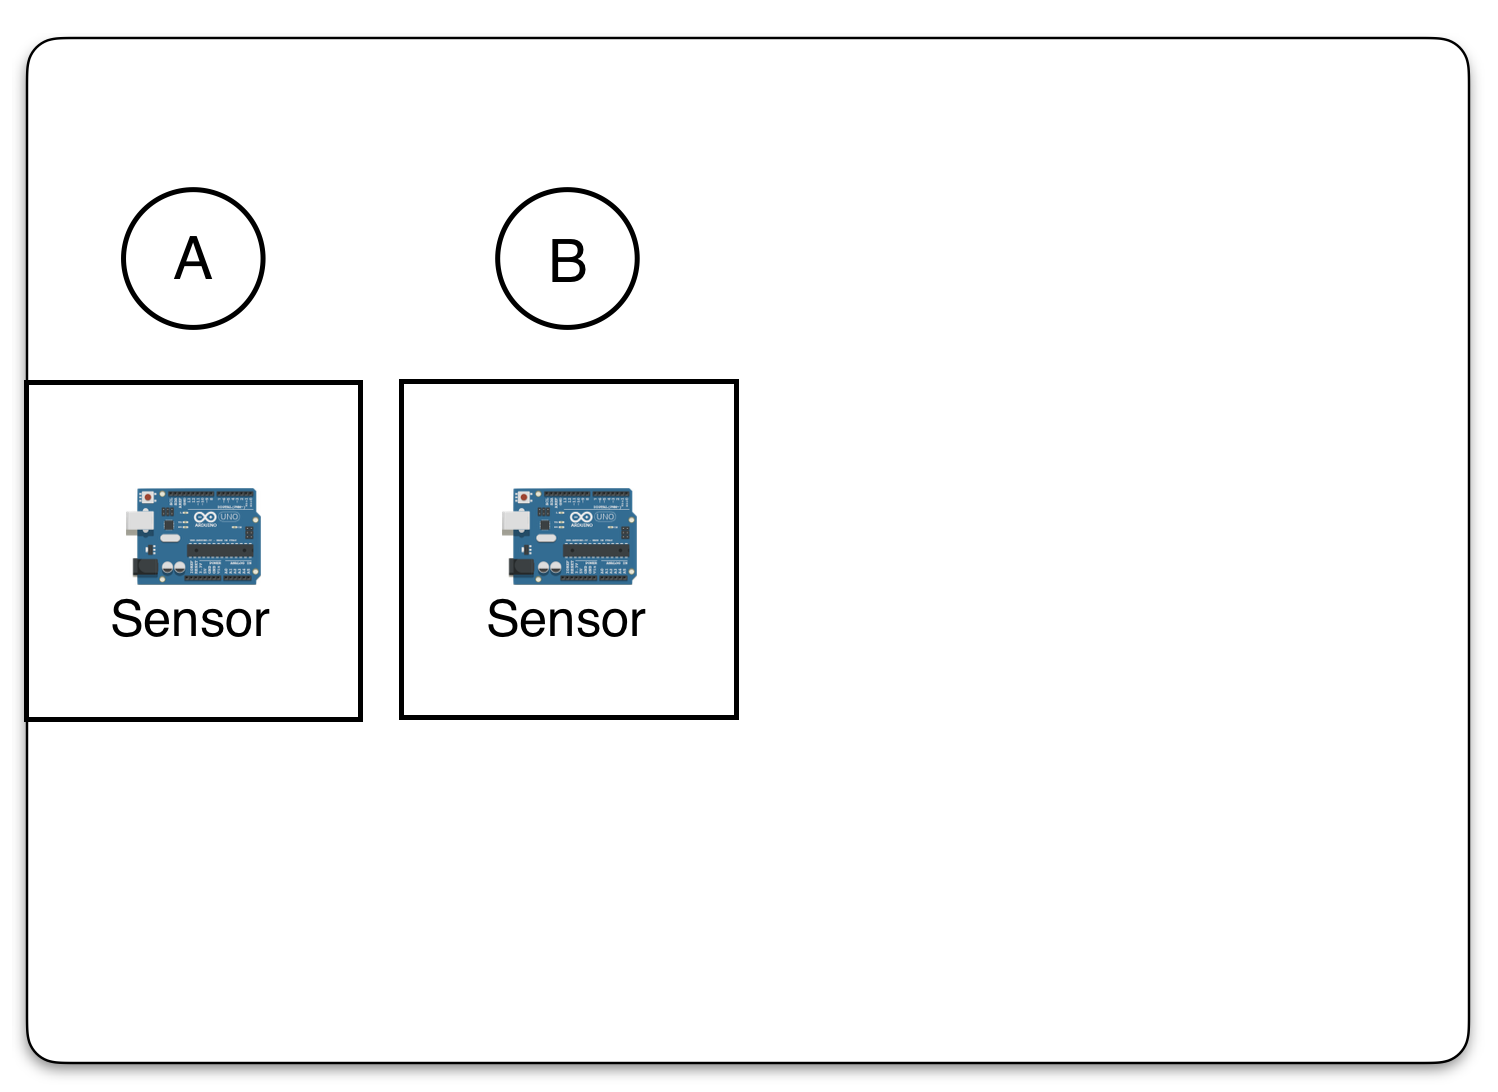
\includegraphics[width=1\linewidth]{figure/scene1.png}
  \caption{study room scene with A and B position}
  \label{fig:Scene}
\end{figure}

\section{Related Work}
There are some existed tools which are related to our work, such as using cameras and infrared sensors to count the number of people in a room\cite{cite4}. This kind of system is installed on the entrance of the room so that it can count the number of people coming in and going out. By getting these numbers, we can easily count the number of people in a room. We want to know how many people are using the table but this kind of system can only tell us the number of people in a room. In many cases people just walk in a room to find their friends, chat a little while and then leave the room. But we want to reflect the real usage of a room and that's why we want to build this system. Although using camera is good way to count the number of people, it might raise some privacy concerns.

There is another research related to our work which is called Building Occupancy Estimation System\cite{cite1}. It uses some sensors on the ground to detect the footsteps and use these data to calculate the number of user in a room. This idea is quite cool but in our situation, students will be studying in the room and they will not move for a long time so it does not work in our case.

We also think of putting pressure sensor on each chair. This is an naive and most accurate way to detect people. But we have to put the sensors on every chair in the campus, this is too costly. We want to minimize the number of sensors we have to use. Therefore we choose to put sensors on each table. If we can detect how many people are using one table, then we can use this device on any kind, any size of the table.

\section{System Design}
Our system detects a table event caused by natural human actions on a table, such as typing keyboards, hitting elbows and flipping pages of books, and estimates human presence at the table. The sensing platform is designed with a data collection board and several piezoelectric sensors. In the signal processing stage, there are two separate modules in our system: table event detection and human presence estimation. First, vibration sensor data are fed into the table event detection module, which determines whether the current data contains a table event potentially caused by human behavior at the table. Every certain period, human presence at the table is evaluated by using table events caused during this period. This module estimates only whether at least one person uses the table. Finally, the people counting module estimates the number of people using the same table. These signal processing modules are implemented using MATLAB.

\subsection{Vibration Sensing Platform}
Figure~\ref{fig:DataCollection} shows the data collection board with a piezoelectric sensor in our vibration sensing platform. In our sensing platform, up to three sensors are connected to the data collection board, enabling us to collect data synchronously. To greatly improve its sensitivity, we used epoxy to glue a mass to each piezo sensor. Additionally, the piezoelectric signals are amplified and filtered by a first order active filter based on an operation amplifier. The amplification gain is 50X so that the small signals caused by human actions such as typing a keyboard is amplified enough to be detected. The low pass filter is designed for anti-aliasing, setting cutoff frequency at 160 Hz. The data collection board is based around the arduino UNO.

\subsection{Table Event Detection}
The table event detection module collects time series of vibration signals from a sensor mounted on the table and determines whether a table event occurred. The system first remove offsets from raw sensor data streams and extracts a signal energy within a time window. The signal energy feature is defined as the sum of the squared values within the time window, which is chosen around 0.2 seconds. The algorithm to determine a table event is based on an anomaly detection model used in several works\cite{cite1}. In this algorithm, the current window's signal energy is compared to a Gaussian noise model for anomaly detection. If the signal energy exceeds three standard deviations above the mean of the noise, the system identifies it as a table event. The system updates the noise parameters based on streamed non-event data in order to continuously adjust changing environments.


\begin{figure}
  \centering
  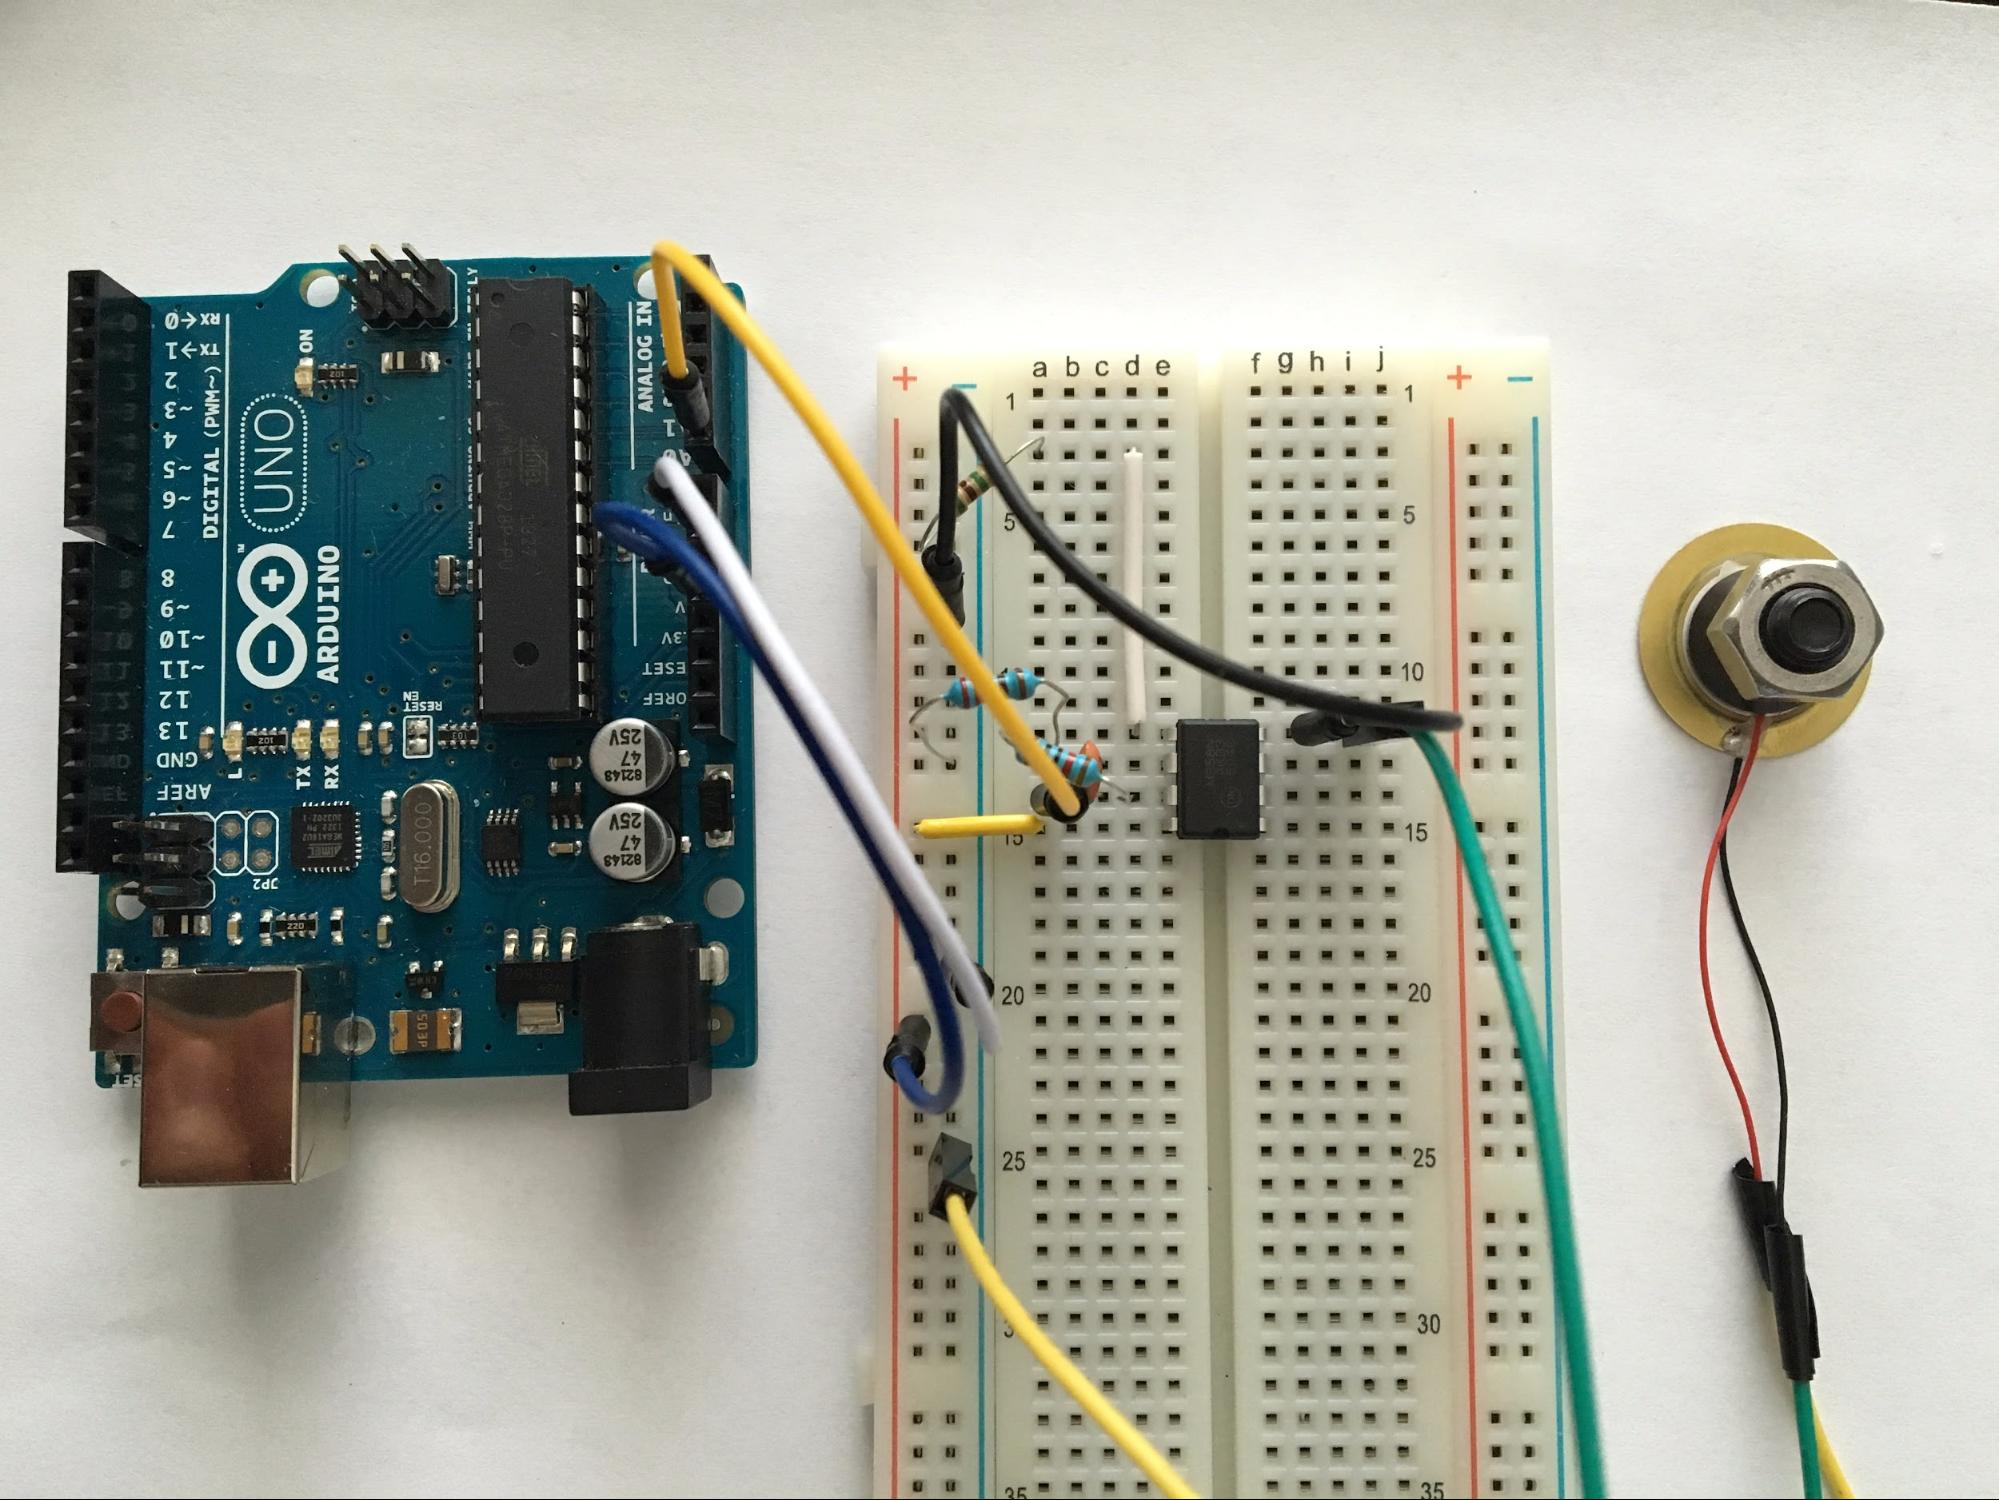
\includegraphics[width=1\linewidth]{figure/dataCollection.jpg}
  \caption{Hardware for data collection}
  \label{fig:DataCollection}
\end{figure}

\subsection{Human Presence Estimation}
Table events does not always necessarily continue to be caused by human presence at the table. In addition, it is possible that other human actions, such as walking near the table, also generates a table event. To estimate correctly human presence at the table, we developed three models to determine whether at least one person is present at the table. 
The first model is sequential detection model (SD), which simply considers sequential table events occurred twice in a row to be human presence. Once a sequential event happens, the system holds the human-present state for a certain period. While holding the present state, if a table event is detected, the holding period is updated. If there is no events occurred in the period, the system changes its state to the absent state. 

The second model, event counting model (EC), computes the number of table events generated in a certain period, comparing the count to a threshold. If the event count is beyond the threshold, the system considers the state present. If it is below the threshold, the state is regarded as absence.

The third model, filtered event counting model (FEC), is based on the second model EC. The only difference from EC is that the system ignores a table event occurred simultaneously at the different neighboring tables. This model is aimed for reducing error events caused by footsteps or any other actions not in the corresponding tables. Since the propagation speed of footsteps through the floor medium is much faster than the sampling rate, we assume that a table event caused by a footstep at the different tables in the same room are synchronized. The tradeoff is that it can also eliminate signals caused by actions at one table propagating to the other tables. But in normal situations, people will not generate signals large enough to propagate to another table. Therefore, we can assume the synchronized signals are all something big like footsteps or slamming the door so that eliminating these signals will be reasonable. 


\begin{figure}
  \centering
  \includegraphics[width=1\linewidth]{figure/systemDescrition.pdf}
  \caption{System Descrition}
  \label{fig:SystemDescrition}
\end{figure}



\section{Experiment Method}
\subsection{Experiment: Study Room Student Detected}

In this experiment, we are going to detect whether there is any student in the study room. We put the vibration sensor with sampling frequency 1kHz and connect it with Arduino UNO board embedded in the central of each table in the room. In addition, we try to find out a threshold value in order to eliminate the environment vibration from other sources, such as the door opening/closing, or other students in the same room. For example, if the vibration value we detected is larger than the threshold, we would consider it as a student existed on this table, otherwise would be taken as the environment disturbance and not be counted as a student. 


Additionally, in general cases, one study room would have not only one table for student to use, which may cause additional vibration detected on a table's sensor from the nearby tables. For instance, although table A has no student usage, the nearby table with one student uses at the same time would also create the vibration to the table A. This vibration caused by nearby table must be smaller than the vibration created by table A' user. Therefore, we also view this vibration as environment disturbance with value lower than threshold and ignore it.

As we can see in Table \ref{tab:table1}, we perform our experiment in four scenario with two experiment study table in one room. The first scenario shows that both tables are absent with one manual vibration produced. With this scenario, we can know the basic environment vibration signal for our environment vibration elimination purpose. 
The second scenario has two absent table with one student using PC on the third table. In this case, the environment disturbance would enhance significantly compared to the first scenario. However, with the first two scenario, we can know the pattern of the environment vibration signal which we should eliminate in our experiment. The third scenario shows that one table absent while another table has one student who is using PC, and the last scenario indicates that both tables have students using PC at the same time. With the third and fourth scenario, we can know the vibration volume while students are using study table in general cases.

\begin{table}
    \centering
    \caption{Experimental Condition with Sampling frequency 1kHz}
    \begin{tabular}{|c|l|l|l|}
      \hline
      \tabhead{\#} &
      \multicolumn{1}{|p{0.1\columnwidth}|}{\centering\tabhead{Table 1}} &
      \multicolumn{1}{|p{0.1\columnwidth}|}{\centering\tabhead{Table 2}} &
      \multicolumn{1}{|p{0.45\columnwidth}|}{\centering\tabhead{Remarks}} \\
      \hline
      1 & absent & absent & N/A \\
      \hline
      2 & absent & absent & sb at Table 3 using PC(~5 m)\\
      \hline
      3 & absent & present & using PC\\
      \hline
      4 & present & present & both using PC\\
      \hline
    \end{tabular}
    
    \label{tab:table1}
  \end{table}

% \begin{figure}
% \centering
% 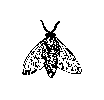
\epsfig{file=fly.eps}
% \caption{A sample black and white graphic (.eps format).}
% \label{fig:example}
% \end{figure}


\begin{table*}[h]
  \centering 
  \caption{The statistical parameter of event counts and the performance of SE, EC, and FEC in each experimental condition}
  \begin{tabular}{|c|c|c|c|c|c|c|}
    \hline
    \multirow{4}{*}{Conditions} &
      \multicolumn{2}{c|}{\multirow{3}{*}{Event Counts/minute}} &
      \multicolumn{3}{c|}{\multirow{3}{*}{Rate of Human Presence}} & 
      \multirow{4}{*}{Total Time(minutes)} \\
      &\multicolumn{2}{c|}{}&\multicolumn{3}{c|}{}&\\
      \cline{2-6}
        & Mean & SD & SE & EC & FEC & \\ 
      \hline
      1 & 1.2 & 1.8 & 0.06 & 0.00 & 0.00 & 20\\
      \hline
      2 & 7.4 & 10.7 & 0.58 & 0.11 & 0.17 & 50\\
      \hline
      3 & 11.6 & 14.2 & 0.73 & 0.14 & 0.07 & 40\\
      \hline
      4 & 75.6 & 50.5 & 0.99 & 0.98 & 0.98 & 130\\
      \hline
  \end{tabular}
  \label{tab:table2}  
\end{table*}


\begin{figure*}[h]
  \centering
  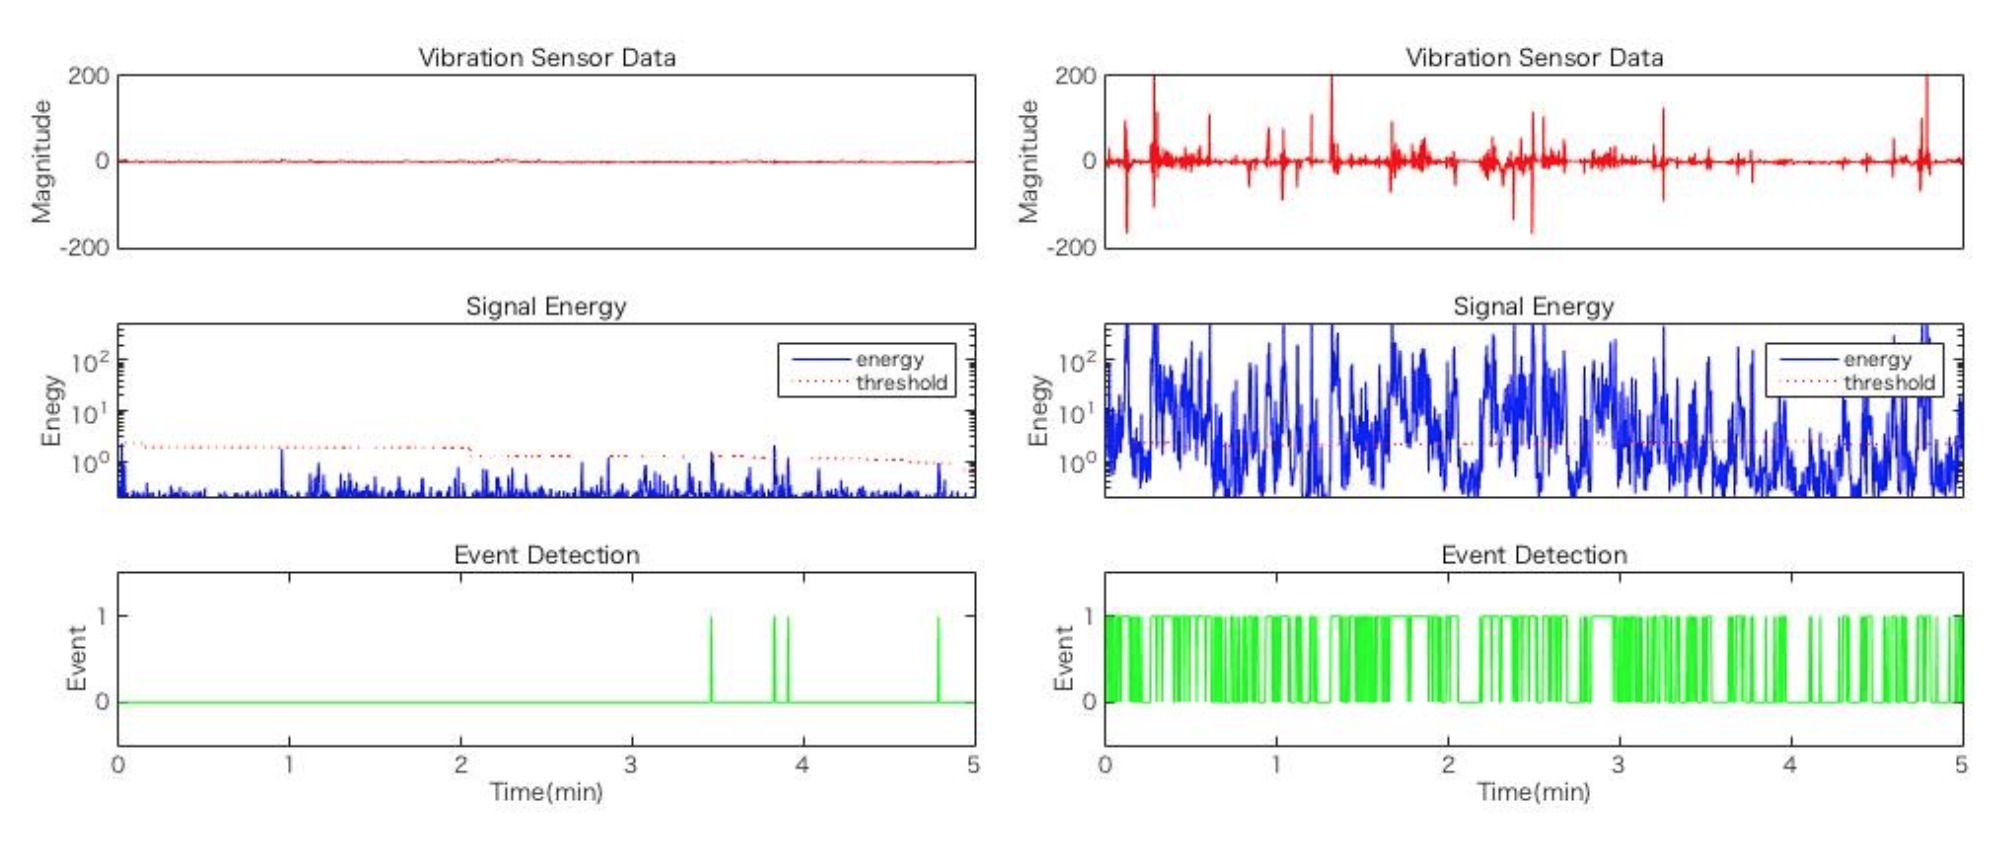
\includegraphics[width=1\linewidth]{figure/result12.pdf}
  \caption{Vibration, energy, and event data for absent-state (left) and present-state (right)}
  \label{fig:Result12}
\end{figure*}


\section{Result}

In this section, the performance of our system is evaluated. The evaluation is based on experimental results.

\subsection{Event Detection}
Figure~\ref{fig:Result12} presents typical data we obtained in the present and absent condition: vibration readings from sensing platform, signal energy and table events computed with the event detection module. While the present and absent state is clearly distinguished in the figure, we found that human footsteps can produce significant noise vibrations at tables in the same room. In four experimental conditions, we performed event detection and evaluated the mean of event counts per minute and its standard deviation (shown in Table \ref{tab:table2}). Even if the table is conditioned absent, somebody working something at a short distance from the table, such as using PC at other tables, produces significant amount of table events in error.


% \begin{figure}
%   \centering
%   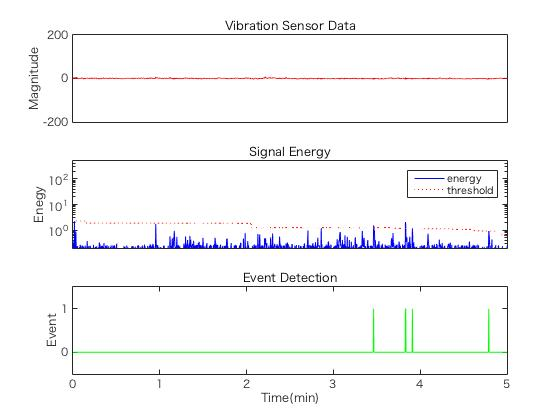
\includegraphics[width=0.8\linewidth]{figure/result1.jpg}
%   \caption{Hardware for data collection}
%   \label{fig:Result1}
% \end{figure}

% \begin{figure}
%   \centering
%   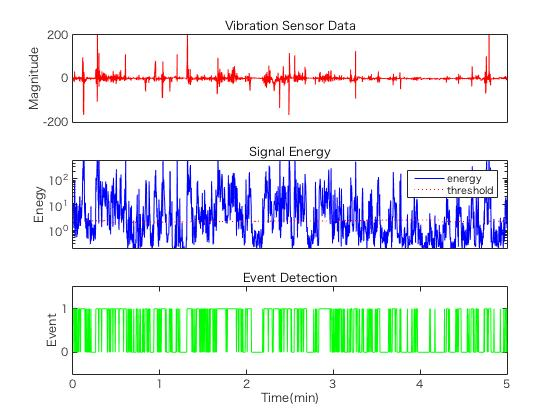
\includegraphics[width=0.8\linewidth]{figure/result2.jpg}
%   \caption{Hardware for data collection}
%   \label{fig:Result2}
% \end{figure}


\begin{figure*}[h]
  \centering
  \includegraphics[width=1\linewidth]{figure/eventCounts.pdf}
  \caption{Event counts and human presence for absent state (left) and present state (right) in condition 3}
  \label{fig:EventCounts}
\end{figure*}

\subsection{Human Presence Estimation}
In order to verify the effectiveness of removing simultaneous events from the event data, the performance of human presence with normal event counting model (EC) and filtered event counting model (FEC) is evaluated. Figure~\ref{fig:EventCounts} shows the results for a absent state table and a present state table in experimental condition 3. The number of table events was counted by 2.5 minutes and compared to the threshold to estimate human presence. As can been seen, with FEC, we can filter the event counts in the absent state and determine the correct state. This result indicates that although vibration caused by some kinds of human behavior at one table, such as footsteps, can propagate to neighboring tables, these kinds of table event is not dominant in natural human activity. However, in extreme case, such as someone stamping the ground or hitting a table frequently, this FEC method might not work well.

The three different models for human presence estimation is compared in performance. Table \ref{tab:table1} presents the rates of the present condition in each room condition, the total time identified as the present state by each model divided by the data collection time. Due to the noise vibration mostly originated from somebody's footsteps, SE model indicates the relatively high present rate in absent table when somebody is working near the table. On the other hand, with EC and FEC model, around 10 percent values are obtained even if somebody is at a distance of one meter from the sensor. While the filtering simultaneous events (FEC) works well in the condition 3, in the condition 2, the value with FEC is worse than that with EC. This implies that there might be some other noise modes that propagates too slow to assume synchronization between neighboring tables.


\section{Future Work}

Detect the number of people who are using the table
Our ultimate goal is to detect the number of people who are using the table. By doing so, we can use this device on any kind of table. For example, we can put it on a larger table like the table in classroom or conference room. Therefore we can estimate number of people who is using that table in the room. There are some possible approaches to reach this goal, we want to try to distinguish the signal from different people by the difference of time arrival. If we would like to choose this approach, we need to increase the sampling frequency. But there are some limitations on the Arduino Uno board. We cannot increase the sampling frequency because the speed of writing data through serial port is too slow and the ram on the board is too small so that we are not able to handle too many data input at the same time. We think we can use a better Arduino board to solve this problem. 

Publish the results
The problem we want to solve is to build a system and let us find a place to study more easily. Therefore after we finish building the sensor system, we can connect all the devices to the Internet. We want to build a server to receive these data and provide a web service to show the results to all the students in the campus. If a student want to find a place to study, then he/she can check our website first and find the most suitable room for himself/herself.

Connect the system to lights and air conditioners
We want to save energy. Hence we have to connect our system to lights and air conditioners. If we detect there is nobody using the room for a predefined period of time, we can turn off the lights and air conditioners to save the energy.



%ACKNOWLEDGMENTS are optional
% \section*{Acknowledgments}
% Acknowledgement goes here.

%
% The following two commands are all you need in the
% initial runs of your .tex file to
% produce the bibliography for the citations in your paper.
\bibliographystyle{abbrv}
\bibliography{sigproc}  % sigproc.bib is the name of the Bibliography in this case
% You must have a proper ".bib" file
%  and remember to run:
% latex bibtex latex latex
% to resolve all references
%
% ACM needs 'a single self-contained file'!
%
%APPENDICES are optional
%\balancecolumns
% \appendix
%Appendix A

% Appendix goes here.

% That's all folks!
\end{document}
